\documentclass[12pt,a4paper]{article}
\usepackage[utf8]{inputenc}
\usepackage[spanish]{babel}
\usepackage{amsmath}
\usepackage{amsfonts}
\usepackage{amssymb}
\usepackage{graphicx}
\usepackage[left=2cm,right=2cm,top=2cm,bottom=2cm]{geometry}
\author{Enciso Guerrero Benjamin Salvador\\
Carlos Enrrique Moran Garabito\\
Cinematica De Robots }
\title{Istalacion de ROS}
\begin{document}
\maketitle

\includegraphics[scale=1.8]{practica1garabito/upzmgg.jpg} 
\newpage
Instalacion de ROS.\\\\
Esta nueva versión de ROS fue lanzada primeramente para Ubuntu 16.04 (Xenial), aunque posteriormente se ha buscado compatibilidad con otros sistemas operativos (distribuciones de Linux, OS X, Android y Windows) con distinto grado de soporte.
\\\\
*Configurar el fichero sources.list
\\\\
Lo primero que debemos de realizar es la configuración para que nuestro ordenador acepte software de packages.ros.org. Para ello debemos de introducir en el terminal la siguiente línea:
\\\\
sudo sh -c 'echo "deb http://packages.ros.org/ros/ubuntu
\\\\
*Configurar las keys.
\\\\
El siguiente paso también es copiar una línea en el terminal.\\
Las keys se utilizan en Ubuntu para confiar en los repositorios, por ello es necesario que introduzcamos la correcta.
\\\\
sudo apt-key adv --keyserver hkp://ha.pool.sks-keyservers.net:80 --recv-key 0xB01FA116
\\\\
*Instalación
\\\\
Primero, verificamos que tenemos todos los paquetes actualizados.
\\\\
sudo apt-get update
\\\\
Una vez concluida la actualización pasamos a la instalación de ROS. Existen varios tipos de instalación según lo que necesitemos (versión completa, de escritorio, para máquinas remotas, … ). En nuestro caso instalaremos la versión completa, que además es la recomendada.
\\\\
sudo apt-get install ros-kinetic-desktop-full
\\\\
La instalación nos pedirá permisos para continuar, le diremos que sí (Y).
\\\\
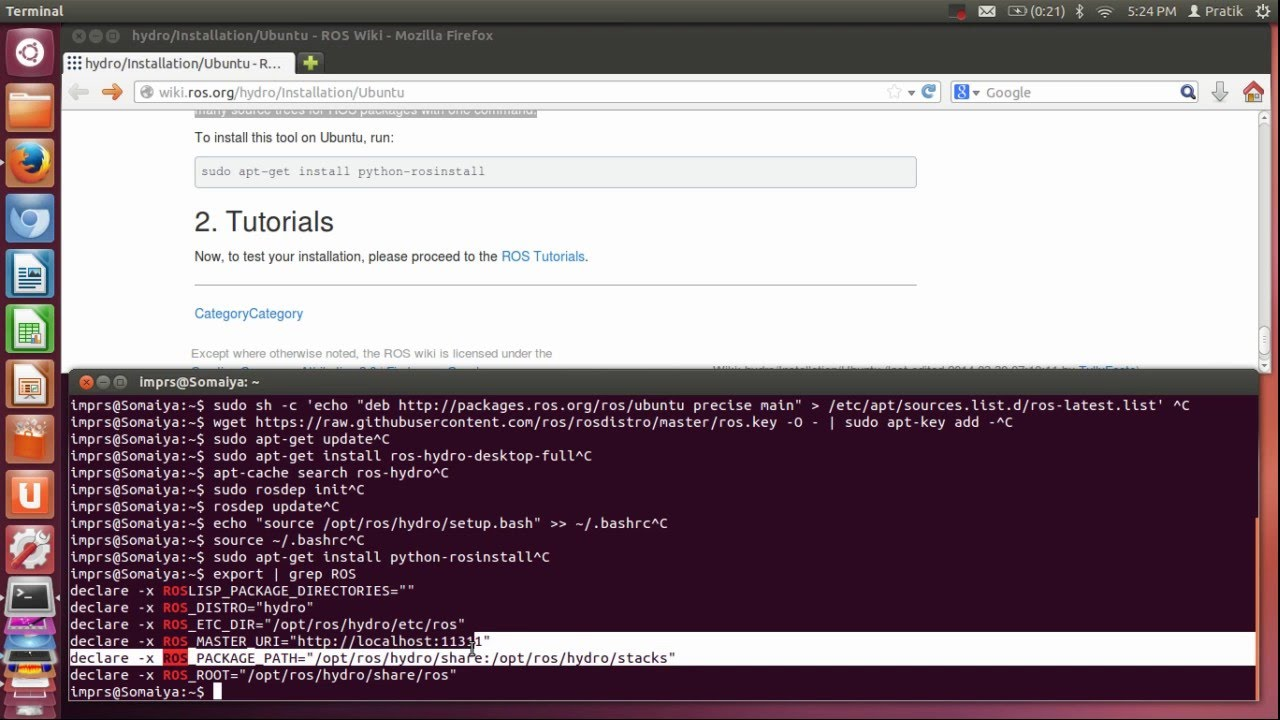
\includegraphics[scale=0.3]{maxresdefault.jpg} 
\\\\
*Inicialización de rosdep
\\\\
Antes de poder usar ROS es necesario inicializar rosdep. Rosdep permite instalar fácilmente dependencias para el código que compilemos y además es requerido por algunos componentes del núcleo de ROS.
\\\\
sudo rosdep init \\
rosdep update
\\\\

*Configuración del entorno
\\\\
Por defecto, el sistema no carga automáticamente las variables del entorno de ROS, pero lo podemos resolver con la siguientes dos líneas cada vez que lanzamos un terminal.
\\\\
echo "source /opt/ros/kinetic/setup.bash" >> ~/.bashrc \\
source ~/.bashrc
\\\\
Sin embargo, es preferible incluir la línea directamente en el bashrc y nos olvidamos de realizar este proceso siempre. \\
Para ello abrimos con nuestro editor de texto favorito el fichero .bashrc y añadimos la siguiente línea al final del todo.
\\\\
source /opt/ros/kinetic/setup.bash
\\\\
*Rosinstall
\\\\
Rosinstall es una herramienta de la línea de comandos que se usa bastante pero que se distribuye por separado de ROS.  Se suele utilizar sobre todo para descargar de una manera sencilla paquetes de ROS que tienen bastantes ramas con un único comando.
\\\\
sudo apt-get install python-rosinstall
\\\\
*Creación del entorno de trabajo (workspace):
\\\\
En este punto ya tenemos instalado y configurado nuestra versión de ROS, vamos a ver ahora como crear el entorno de trabajo. \\
El espacio de trabajo por defecto en ROS se denomina catkinws, aunque podemos utilizar cualquier nombre que deseemos. \\
Lo primero es crear un directorio con ese nombre y a su vez uno dentro del mismo que se debe de llamar src. 
\\\\
Una vez creados los directorios, entramos en el src y ejecutamos el comando que inicializa el workspace. Veremos además como se crea un fichero  CMakeLists.txt. 
\\\\
\newpage 
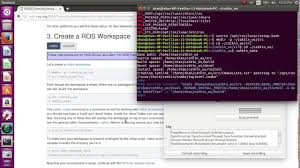
\includegraphics[scale=1.6]{images.jpg} 
\\\\
Y con esto ya podemos empezar a crear nuestros paquetes dentro del directorio src y compilar desde el nivel superior con el comando catkin.make.
\newpage
\title{CONCLUSION.} 
\\\\
ROS es una opción mundial para el avance de la programación robótica. Resulta importante desarrollar competencias en el manejo de tal sistema, yaque si se quiere, en un futuro, presentar propuestas a problemas concretos como el atinente al manejo adecuado de drones con diferentes propósitos, en este caso ROS nos servira para  la simulacion de nuestro proyecto de brazo robotico, resulta de gran importancia usar a la perfección este tipo de herramientas sin mencionar que se encuentra en constante  desarrollo y evolucion.
\\\\
 Al ejecutar "sudo apt-get update" me marco un error. AL hacerlo desde una máquina virtual con Xubuntu 16.04 teniendo que desactivar las superposiciones.
























\end{document}